%%%%%%%%%%%%%%%%%%%%%%%%%%%%%%%%%%%%%%%%%%  不使用 authblk 包制作标题  %%%%%%%%%%%%%%%%%%%%%%%%%%%%%%%%%%%%%%%%%%%%%%
%-------------------------------PPT Title-------------------------------------
\title{\ch{Ni}表面\ch{CO2}的吸附}
%-----------------------------------------------------------------------------

%----------------------------Author & Date------------------------------------
%\author[\textrm{Jun\_Jiang}]{姜\;\;骏\inst{}} %[]{} (optional, use only with lots of authors)
%% - Give the names in the same order as the appear in the paper.
%% - Use the \inst{?} command only if the authors have different
%%   affiliation.
\institute[BCC]{\inst{}%
%\institute[Gain~Strong]{\inst{}%
\vskip 0pt 北京市计算中心有限公司~材料计算团队}
%\vskip -20pt {\large 格致斯创~科技}}
\date[\today] % (optional, should be abbreviation of conference name)
{	%{\fontsize{6.2pt}{4.2pt}\selectfont{\textcolor{blue}{E-mail:~}\url{jiangjun@bcc.ac.cn}}}
\vskip 45 pt {\fontsize{8.2pt}{6.2pt}\selectfont{%北京科技大学% 报告地点
	\vskip 5 pt \textrm{2024.07.30}}}
}

%% - Either use conference name or its abbreviation
%% - Not really information to the audience, more for people (including
%%   yourself) who are reading the slides onlin%%   yourself) who are reading the slides onlin%%   yourself) who are reading the slides onlineee
%%%%%%%%%%%%%%%%%%%%%%%%%%%%%%%%%%%%%%%%%%%%%%%%%%%%%%%%%%%%%%%%%%%%%%%%%%%%%%%%%%%%%%%%%%%%%%%%%%%%%%%%%%%%%%%%%%%%%
\subject{}
% This is only inserted into the PDF information catalog. Can be left
% out.
%\maketitle
\frame
{
%	\frametitle{\fontsize{9.5pt}{5.2pt}\selectfont{\textcolor{orange}{“高通量并发式材料计算算法与软件”年度检查}}}
\titlepage
}
%-----------------------------------------------------------------------------

%------------------------------------------------------------------------------列出全文 outline ---------------------------------------------------------------------------------
%\section*{}
%\frame[allowframebreaks]
%{
%  \frametitle{}
%%  \frametitle{\textcolor{mycolor}{\secname}}
%  \tableofcontents%[current,currentsection,currentsubsection]
%}
%在每个section之前列出全部Outline
%类似的在每个subsection之前列出全部Outline是\AtBeginSubsection[]
%\AtBeginSection[]
%{
%  \frame<handout:0>%[allowframebreaks]
%  {
%    \frametitle{Outline}
%%全部Outline中,本部分加亮
%    \tableofcontents[current,currentsection]
%  }
%}

%-----------------------------------------------PPT main Body------------------------------------------------------------------------------------
\small
\begin{frame}[allowframebreaks]
	\frametitle{文献简介}
	文献\cite{NatCom10-1_2019}\\\textrm{Understanding carbon dioxide activation and carbon–carbon coupling over nickel}%\\(\url{https://doi.org/10.1038/s41467-019-12858-3})}\\
	和文献文献\cite{ASS603-154398_2022}\\
	\textrm{The effect of Ru-Ru coordination numbers on CO 2 methanation over Ru supported catalyst}
	\\分别详尽地讨论了\textrm{\ch{CO2}}在金属\textrm{\ch{Ni}}和\textrm{\ch{Ru}}表面的吸附与反应
	\begin{itemize}
	 \setlength{\itemsep}{-10pt}
		\item 实验结果:~\textrm{\ch{CO2}}在\textrm{\ch{Ni}}表面易生成\textrm{\ch{CH4}}
\begin{figure}[h!]
%\vspace*{-0.18in}
\centering
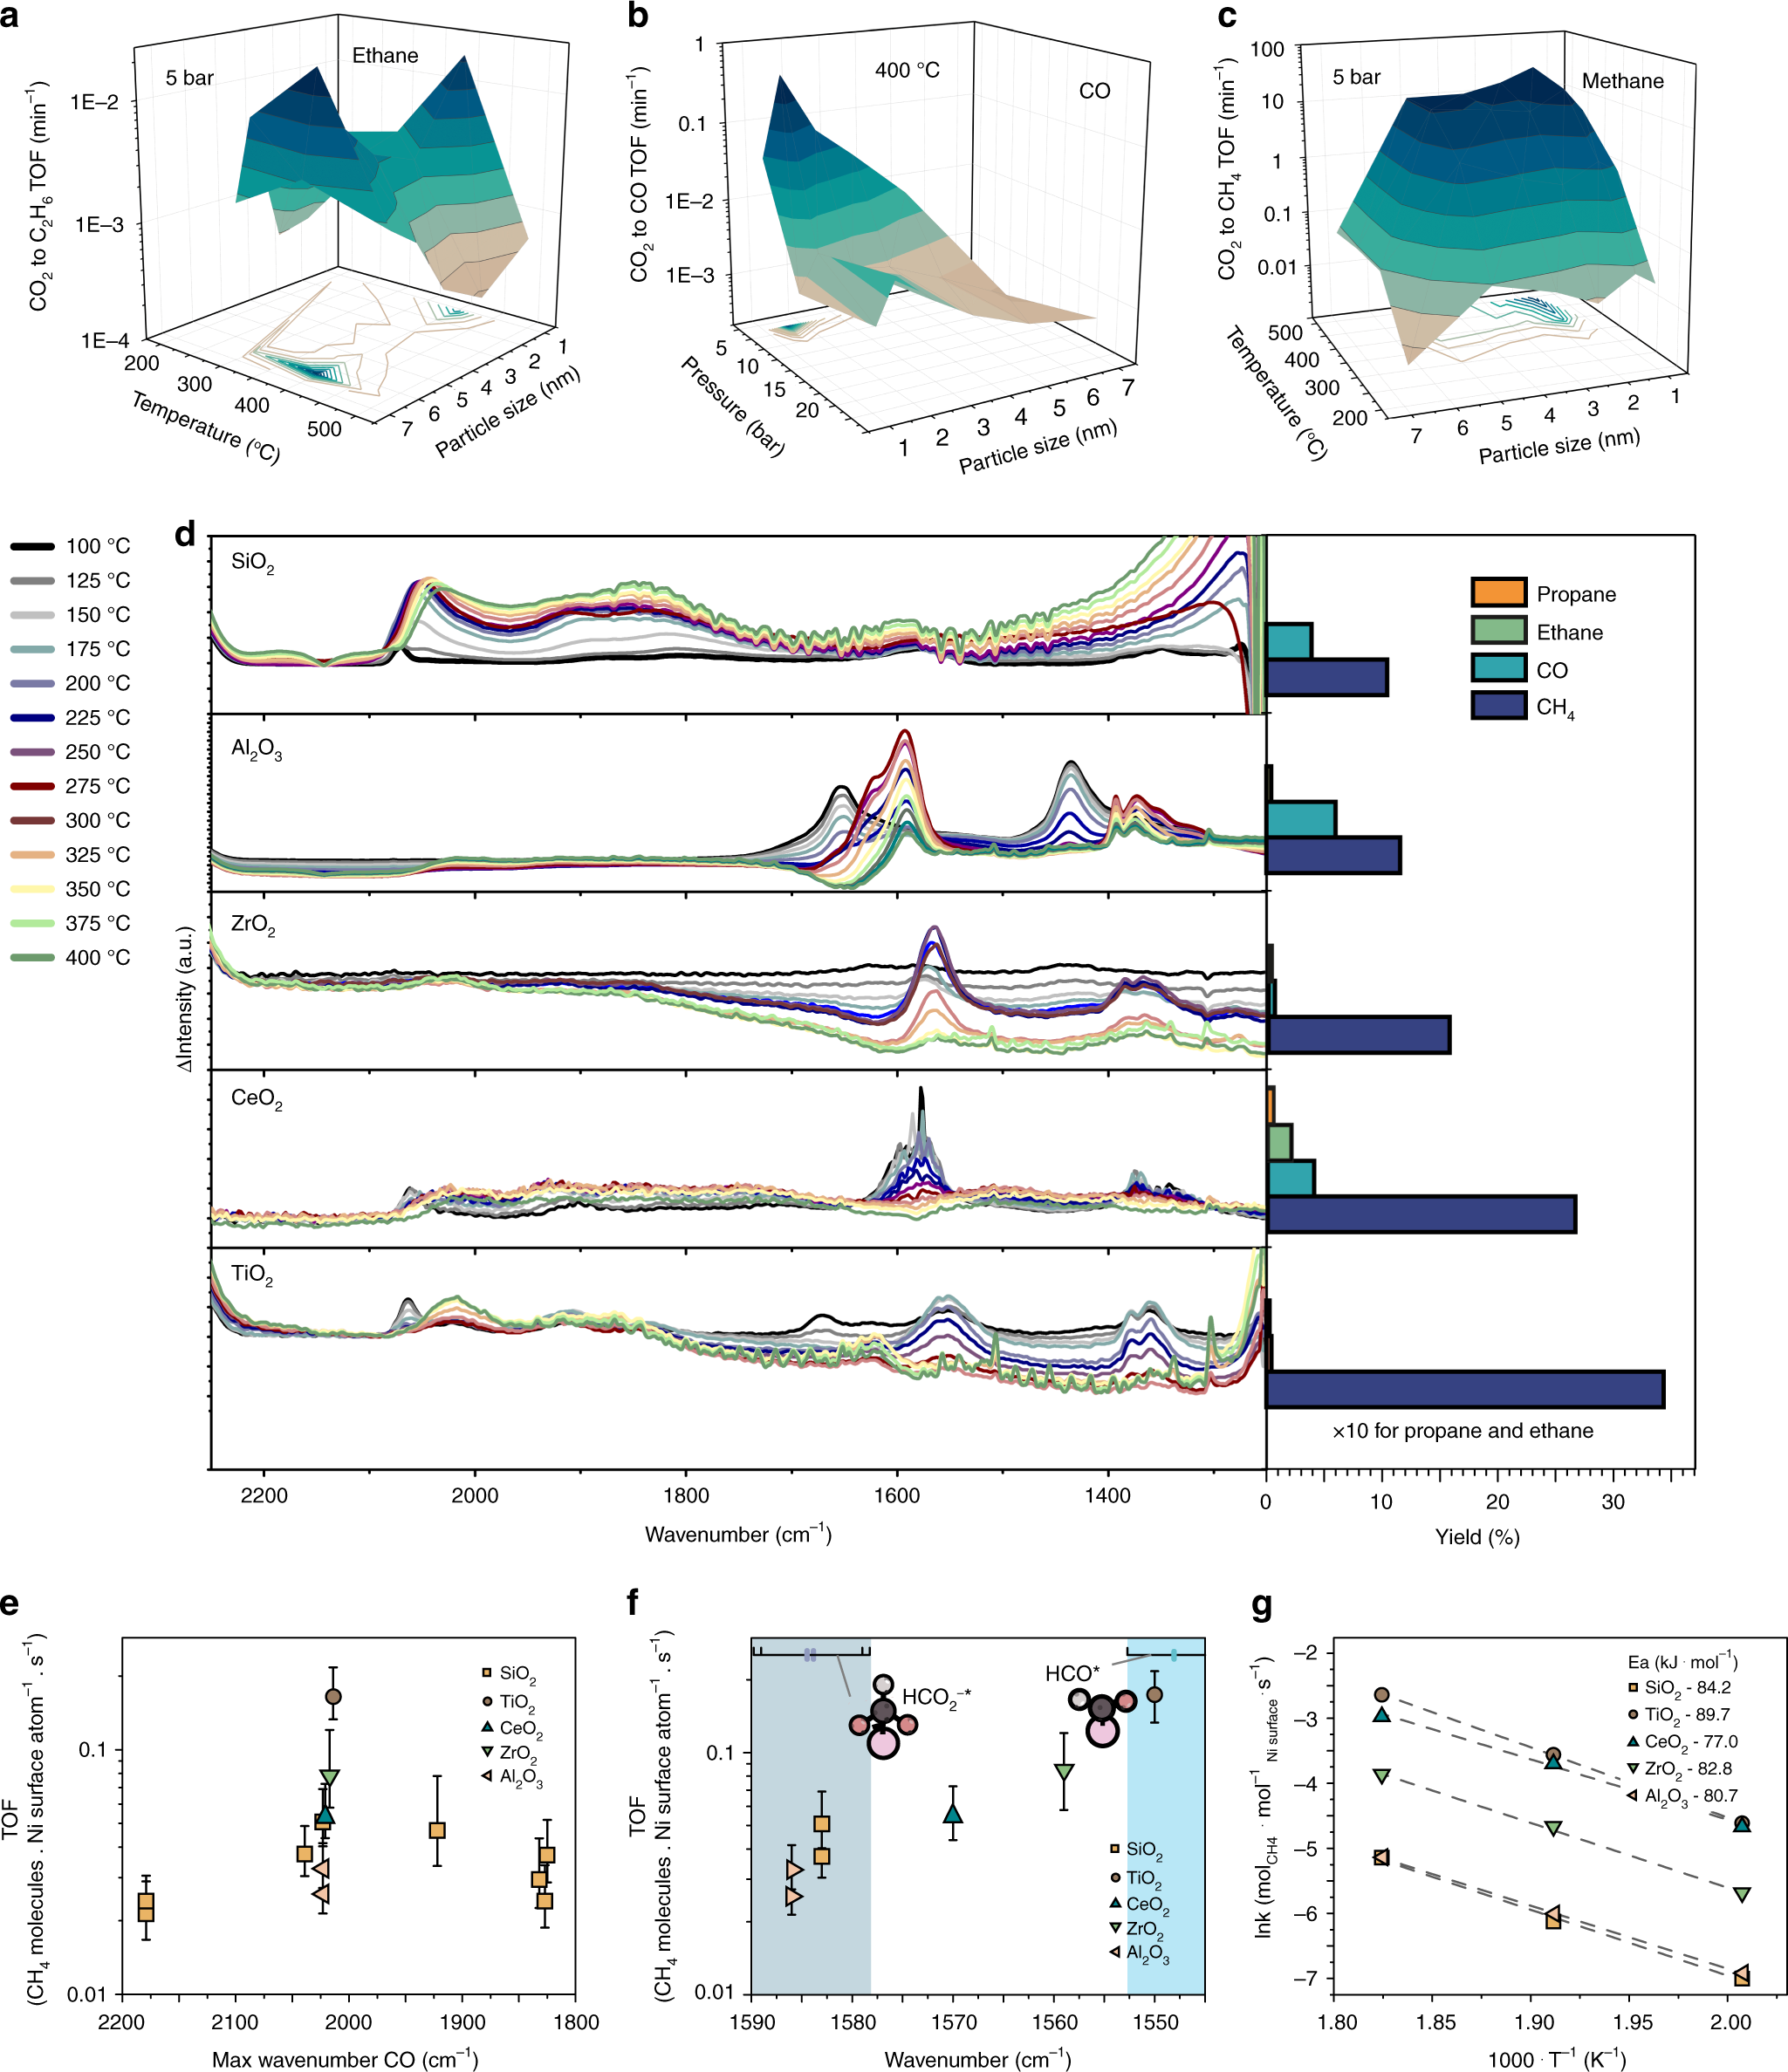
\includegraphics[height=1.50in,width=1.42in]{Figures/CO2_on_Ni-0.png}
\caption{\tiny \textrm{Structure sensitivity and support effects for tuning selectivity and activity in the carbon dioxide hydrogenation over \ch{Ni}.}}%(与文献\cite{EPJB33-47_2003}图1对比)
\label{CO2_0n_Ni-0}
\end{figure}
		\item 理论计算:~\textrm{\ch{CO2}}在金属表面的可能机理
\begin{figure}[h!]
\centering
%\vskip -0.30in
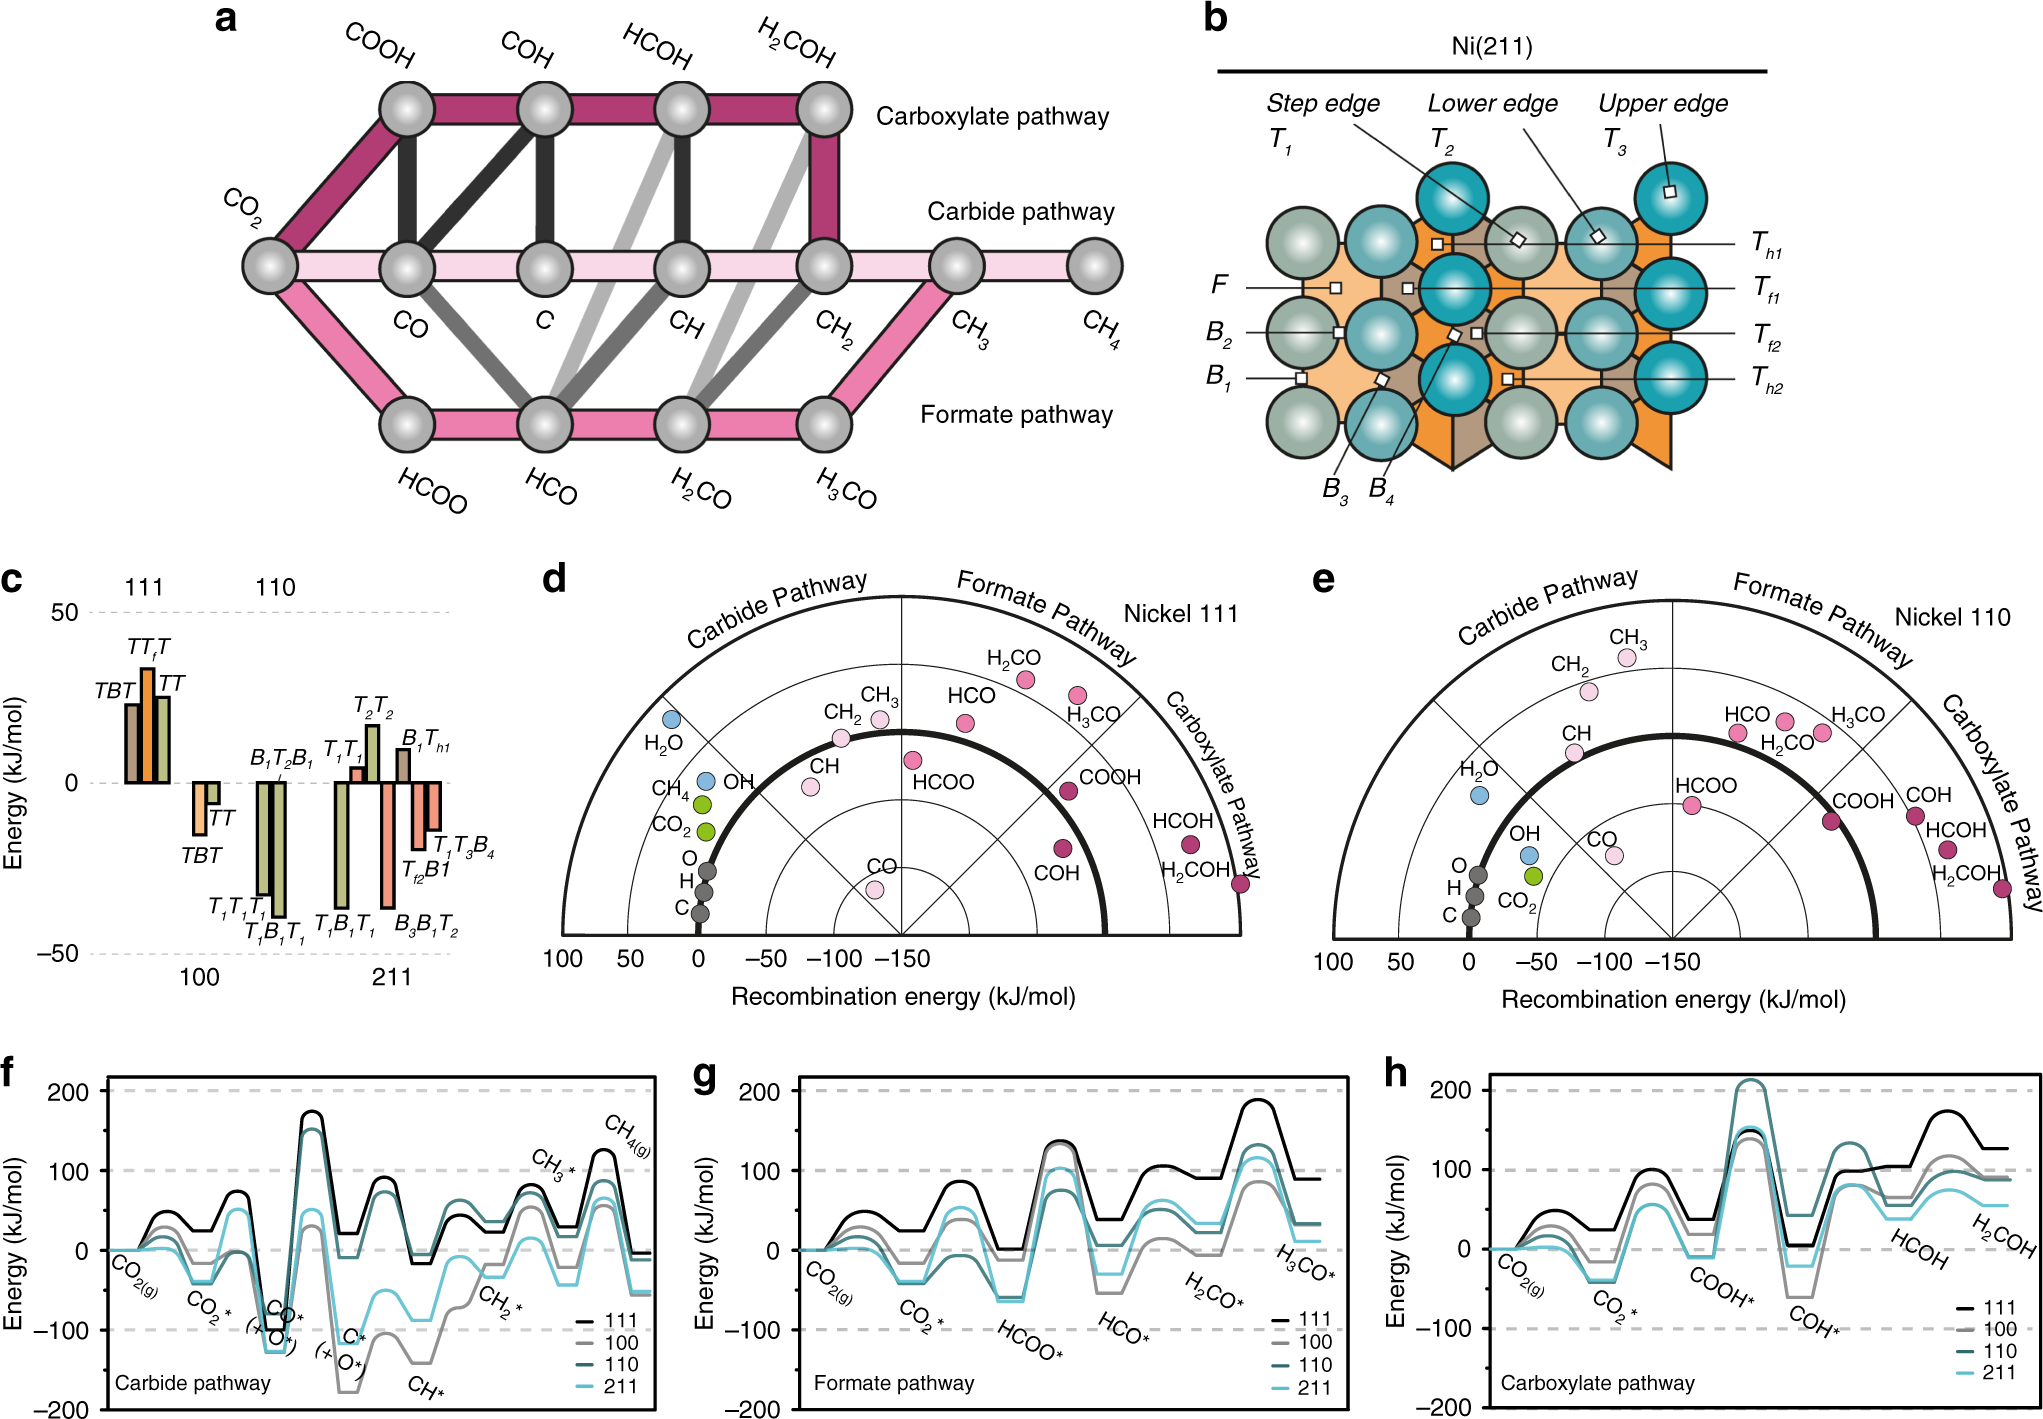
\includegraphics[height=1.60in,width=2.25in]{Figures/CO2_on_Ni-1.png}
\includegraphics[height=0.50in,width=2.12in]{/home/jun-jiang/Pictures/Screenshot from 2024-07-31 11-07-56.png}
\caption{\tiny \textrm{Theoretical calculations of \ch{CO2} activation over \ch{Ni} and \ch{Ru}.}}%(与文献\cite{EPJB33-47_2003}图1对比)
\label{CO2_0n_Ni-1}
\end{figure}
	\end{itemize}
\end{frame}

\begin{frame}
	\frametitle{文献比照}
	计算结果显示
	\begin{itemize}
		\item \textrm{\ch{CO2}}在\textrm{\ch{Ni}}表面易分解为\textrm{\ch{CO}}:\\
			\textrm{\ch{CO2}}在\textrm{\ch{Ni}}表面更易形成~\textcolor{red}{\textrm{\ch{HCOO}}}和~\textcolor{red}{\textrm{\ch{COOH}}}
		\item \textrm{\ch{CO}}经过加\textrm{\ch{H}},脱\textrm{\ch{O}}产生\textrm{\ch{CH4}}\\
			\textrm{\ch{CO}}与\textrm{\ch{H}}形成~\textcolor{red}{\textrm{\ch{HCO}}}
	\end{itemize}
	我们的计算结果
\begin{figure}[h!]
%\vspace*{-0.10in}
\centering
\includegraphics[height=1.70in,width=1.05in]{/home/jun-jiang/Pictures/Screenshot from 2024-07-30 14-28-51.png}
\includegraphics[height=1.70in,width=1.05in]{/home/jun-jiang/Pictures/Screenshot from 2024-07-30 14-28-17.png}
%\caption{\tiny \textrm{Theoretical calculations of \ch{CO2} activation over \ch{Ni}.}}%(与文献\cite{EPJB33-47_2003}图1对比)
\label{CO2_0n_Ni-CO}
\end{figure}
\end{frame}

\begin{frame}
	\frametitle{文献比照}
	文献\cite{ASS603-154398_2022}给出\textrm{\ch{CO2}}在\textrm{\ch{Ru}}表面反应的活化能
\begin{figure}[h!]
\centering
%\vskip -0.20in
\includegraphics[height=1.30in,width=2.45in]{/home/jun-jiang/Pictures/Screenshot from 2024-07-31 11-07-28.png}
\includegraphics[height=1.30in,width=1.60in]{/home/jun-jiang/Pictures/Screenshot from 2024-07-31 11-08-03.png}
%\caption{\tiny \textrm{Theoretical calculations of \ch{CO2} activation over \ch{Ni}.}}%(与文献\cite{EPJB33-47_2003}图1对比)
\label{CO2_0n_Ru-CO}
\end{figure}

\end{frame}
\begin{frame}
	\frametitle{后续计算结果}
	\begin{itemize}
		\item 文献和我们的计算表明,甲醛基~\textrm{(\ch{HCO}$\cdot$)}的生成应该在\textrm{\ch{CO}}产生之后;~初始反应时,甲醛基~\textrm{(\ch{HCO}$\cdot$)}的生成比甲酸基~\textrm{(\ch{HCOO}$\cdot$)}和羧酸基~\textrm{($\cdot$\ch{COOH})}困难
		\item 
			\begin{enumerate}
				\item 基底吸附\textrm{CO2}的基态能量 $\mathrm{E}_{sub}^{\mathrm{CO_2}}=-1035.594648~\mathrm{eV}$
				\item 反应中间体的基态能量 $\mathrm{E}_{sub}^{\mathrm{\chemfig{C(=[1]O)-OH}}}=-1037.7071~\mathrm{eV}$
				\item 反应中间体的基态能量 $\mathrm{E}_{sub}^{\mathrm{\chemfig{HC(=[1]O)-O}}}=-1038.5303~\mathrm{eV}$
				\item 基底吸附\textrm{CO}的基态能量 $\mathrm{E}_{sub}^{\mathrm{CO}}=-1028.222503~\mathrm{eV}$
			\end{enumerate}
		\item \textcolor{blue}{在\textrm{\ch{CO}}生成及后续反应通道的选择}\\
	计算:~\textcolor{red}{实验关心的反应历程}
	\end{itemize}
\end{frame}
